\documentclass[aspectratio=169]{beamer}              % only frames

% for themes, etc.
\mode<presentation>
\usetheme{Madrid} 
\usecolortheme{crane}

%\usepackage{times}  % fonts are up to you
% The usual suspects
\usepackage{multirow, booktabs, dcolumn, color, graphicx} % Tables\usepackage{graphicx}
\usepackage{amsmath,amssymb,amsthm}
% Strikethrough text
\usepackage{soul}
% Adjust box to fit tabulars
\usepackage{adjustbox}
% Embed video
\usepackage{media9}
% For notes
\usepackage{pgfpages}
%\setbeameroption{hide notes} % Only slides
%\setbeameroption{show only notes} % Only notes
\setbeameroption{show notes on second screen=right} % Both
% Give a slight yellow tint to the notes page
%\setbeamertemplate{note page}{\pagecolor{yellow!5}\insertnote}\usepackage{palatino}
% Use colors by name
\usepackage{xcolor}
% EMBEDDING VIDEO IS POSSIBLE WITH PDFPC USE PDF PC to present
\usepackage{multimedia}



% The table highlighting for hypothesis discussion.
\usepackage[beamer,customcolors]{hf-tikz}
\usetikzlibrary{calc}

% To use background images
\newenvironment{colorframe}[2][]{%
\setbeamercolor{background canvas}{bg=#1}
\begin{frame}\color{white}}
{\end{frame}}


% To set the hypothesis highlighting boxes red.
\tikzset{hl/.style={
    set fill color=red!80!black!40,
    set border color=red!80!black,
  },
}

% Set Graphics folder
\graphicspath{{./figures/}}


% these will be used later in the title page
\title{Common Threats and Solutions}
\subtitle{For the Average Citizen}
\author{Irfan Kanat}
\institute[CBS]{{Department of Digitization}\\ Copenhagen Business School}
\date{\today}



\begin{document}

% this prints title, author etc. info from above
\begin{frame}

	\titlepage

    \vfill
    {\tiny \centering This work is licensed under a \href{http://creativecommons.org/licenses/by/4.0/}{Creative Commons Attribution 4.0 International License}.}

\end{frame}

\note{In the previous modules we learned about privacy, stalking, and surveillance as well as reducing your foot print online to make tracking harder. In this module we will learn about typical threats facing an average citizen and how to improve your security against them. In the previous module our focus was on the network traffic, now our focus will be on device security.}

\begin{frame}
	\frametitle{Common Threats}
    
    \begin{itemize}

        \item Unauthorized Access

        \item Bugs

        \item Malware

        \item Network Access

    \end{itemize}

\end{frame}

\note{

}


\begin{frame}
    \frametitle{Unauthorized Access}

    \centering
    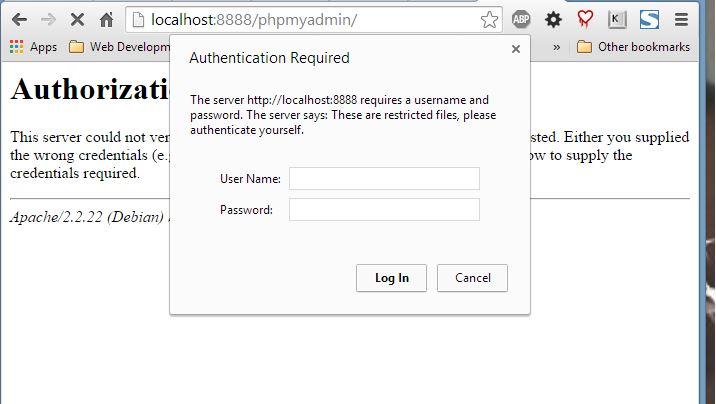
\includegraphics[width = \textwidth, height = .85\textheight, keepaspectratio]{Authentication.jpg}

\end{frame}

\note{
    This is essentially an adversary gaining access to resources they shouldn't have access to. While the topic of unauthorized access is much broader, for a typical citizen in his/her private life it often comes down to authentication.

    Authentication today is mostly done through passwords. Just like it was 40 years ago. It is hard to believe, but we haven't been able to find a better way...

    The adversary can be someone you know, or a malicious third party.

    The way they gain access can be either by guessing your password, trying random passwords until they find the one, tricking you into sharing your password, or using a password you used elsewhere.
}

\begin{frame}
    \frametitle{Passwords are like Underwear}
    
        \begin{columns}
            \begin{column}{0.5\textwidth}
    
                Don't leave them lying around. \vspace{1em}

                Don't share them with others. \vspace{1em}

                Change them often. 
        
            \end{column}
    
            \begin{column}{0.5\textwidth}
    
                
\includegraphics[width = \textwidth, height = .85\textheight, keepaspectratio]{figures/undies.png}
    
            \end{column}
    
        \end{columns}

\end{frame}

\note{
    
    Long story short, treat password like you would treat your underwear.

    Don't write it down.

    Don't tell it to others.

    Don't reuse it in many places.

    Don't pick something that is easy to guess.

    Don't pick meaningful words...

}

\begin{frame}
    \frametitle{Having Memory Problems?}
    
    \centering
    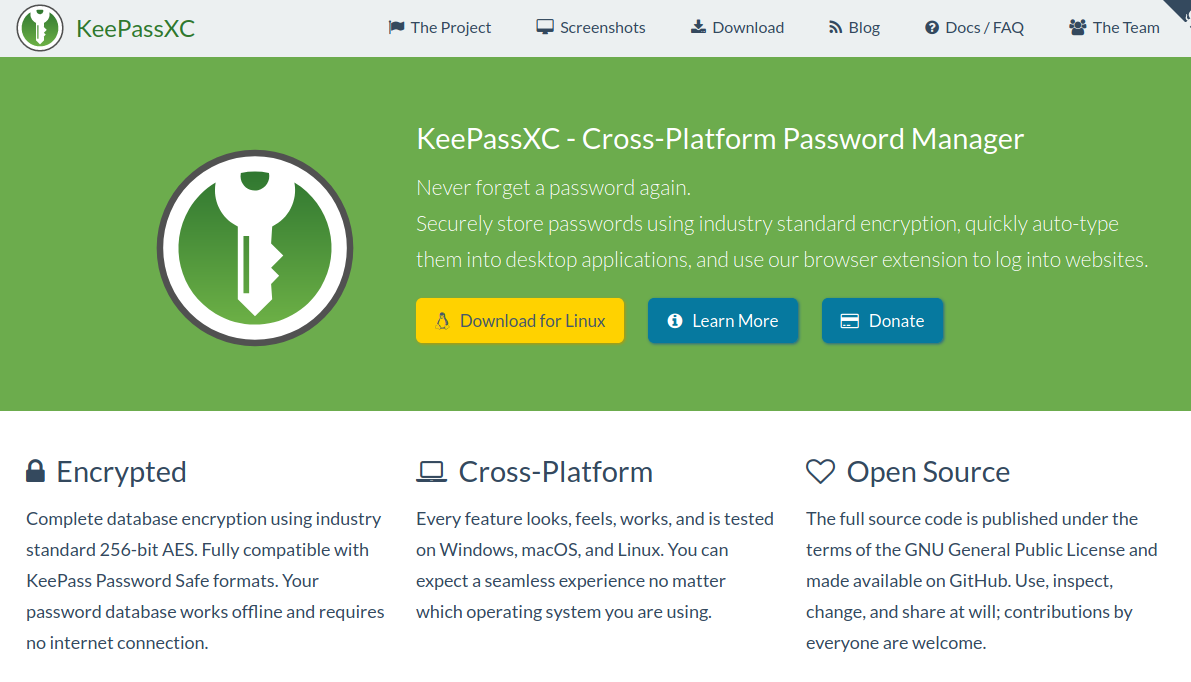
\includegraphics[width = \textwidth, height = .85\textheight, keepaspectratio]{figures/KeepassXC.png}

\end{frame}

\begin{frame}
    \frametitle{Multi Factor Authentication}
    
        \begin{columns}
            \begin{column}{0.5\textwidth}
                    
                \begin{itemize}
                    \item Something You Know
                    \item Something You Are
                    \item Something You Have
                \end{itemize}
        
            \end{column}
    
            \begin{column}{0.5\textwidth}
    
                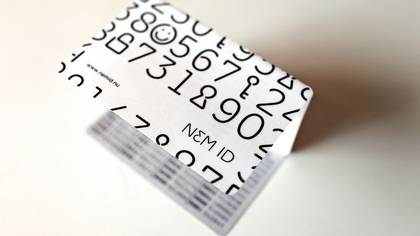
\includegraphics[width = \textwidth, height = .85\textheight, keepaspectratio]{figures/authenticator.jpeg}
    
            \end{column}
    
        \end{columns}

\end{frame}

\note{
    A password is something you know.

    A finger print is something you are.

    A nem id noglekort is something you have.

    Even if adversary gains access to one method of authentication, the other may stump them. Therefore increasing security.
}

\note{A strong password may be hard to remember...

If you follow good advice and use a different password for every site, then that means you need to remember dozens of hard to remember passwords that are not easy to remember...

Solution is to store your passwords in an encrypted repository.

There are some cloud based solutions, but like with everything else, it comes down to trust. Recently a cloud based provider began charging users for access. When that happens, a password manager can be like ransomware.

Therefore I recommend using open source software. You the user will be in control of where your passwords are stored.}

\begin{frame}
    \frametitle{Bugs}
    
        \begin{columns}
            \begin{column}{0.5\textwidth}
    
            Natural \vspace{1em}

            Sometimes can be exploited
        
            \end{column}
    
            \begin{column}{0.5\textwidth}
    
                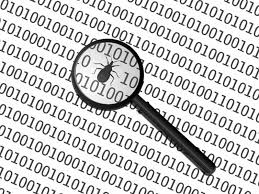
\includegraphics[width = \textwidth, height = .85\textheight, keepaspectratio]{figures/Bug.jpeg}
    
            \end{column}
    
        \end{columns}

\end{frame}

\note{
    Modern software can run into millions of lines of code... The size of the modern software, combined with all the parts that interact with each other make it a very complex endeavor. Akin to designing a jumbo jet...

    This means programmers make mistakes in the code. Some of these won't ever be noticed. Some of the ones we notice, may not harm the daily operation of the system... Others can be used for malicious purposes.

    In worst cases bugs can be used to escalate privilages, meaning the adversary can bypass controls and gain control of the device.
}

\begin{frame}
    \frametitle{Update All Software All the Time}
    
    \begin{itemize}
        \item Update your software regularly.
        \item All of it
        \begin{itemize}
            \item Operating System
            \item Applications
            \item Firmware
        \end{itemize}
    \end{itemize}

\end{frame}

\note{Developers release updates to their software that fixes these bugs.

Once a bug is known, it is easy pickings for attackers.

Therefore it is imperative you keep your system up to date.

One thing you need to know is to stop using hardware and software that no longer receives security updates. This applies to everything: operating systems, applications, cell phones...}

\begin{frame}
    \frametitle{Malware}
        \begin{columns}
            \begin{column}{0.5\textwidth}
    
                \begin{itemize}
                    \item Viruses
                    \item Trojans
                    \item Worms
                    \item Ransomware
                    \item Rootkits
                \end{itemize}
        
            \end{column}
    
            \begin{column}{0.5\textwidth}
    
                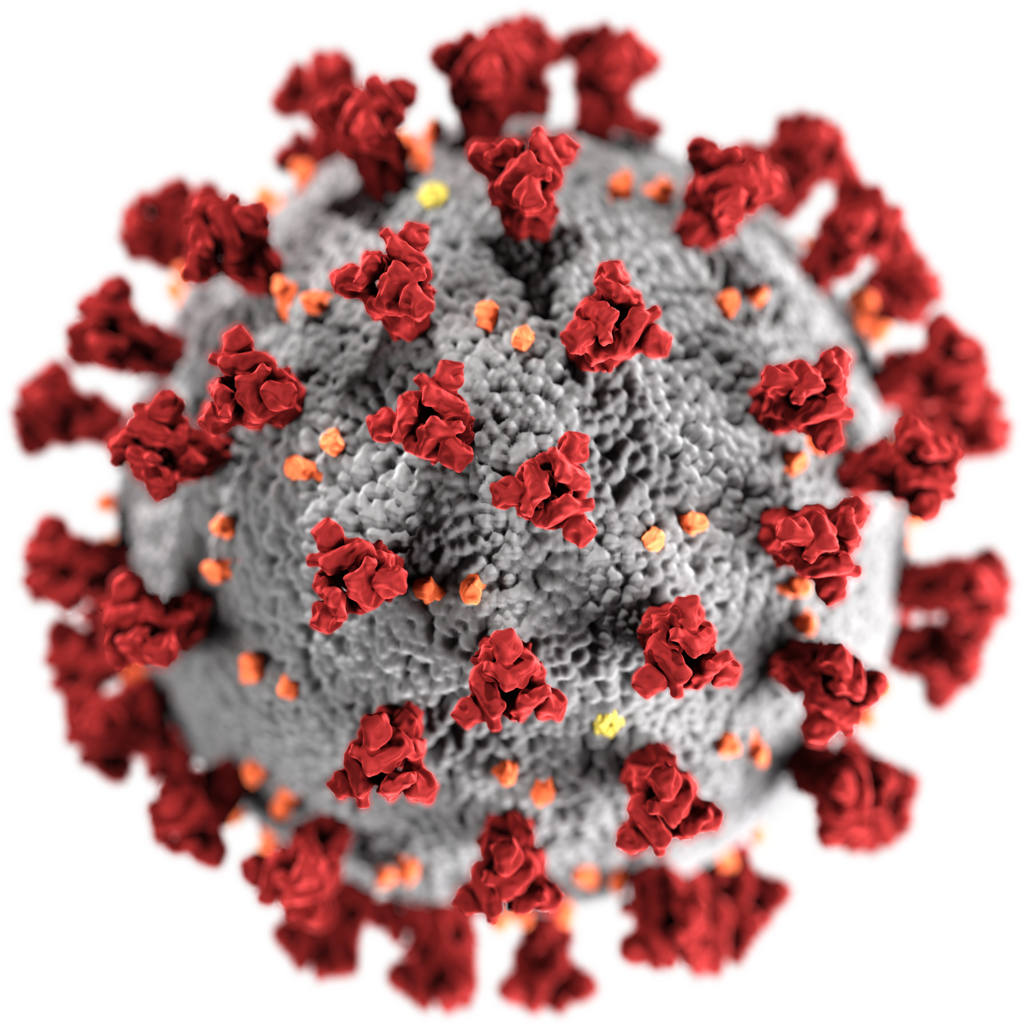
\includegraphics[width = \textwidth, height = .85\textheight, keepaspectratio]{figures/Covid.png}
    
            \end{column}
    
        \end{columns}


\end{frame}

\note{Besides innocent mistakes, there is software written with malicious intent.

Worst of this can spread without user interaction, like NotPetya worm.

But most of it requires user to click a link, open a document, run a program...}

\begin{frame}
    \frametitle{Against Malware}
    
    \begin{itemize}
        \item Update your system.
        \item Update your anti-virus software.
        \item Regularly scan your system.
        \item Don't open files you don't know.
    \end{itemize}

\end{frame}

\note{
    Malware can spread exploiting bugs in your software. Updating your software can protect you against getting infected.

    Anti-virus software can identify and stop known malware. It is important to update virus definitions in your anti-virus software to know your defenses are up to date.

    Most importantly, be careful what you click on. Many web sites on the internet are full of malicious links. As a rule of thumb, don't click or run anything you are unsure about.

    In fact it is often office policy these days to not include or click on any links in any e-mails.

    If a friend for example sent you a file without explanation, ask him what it is through another channel. So if he sent you a file in an e-mail, ask about it over the phone. To make sure it is indeed a legitimate file sent to you.
}

\begin{frame}
    \frametitle{Network Access}

    \centering

    Open Ports + Bugs = Trouble

    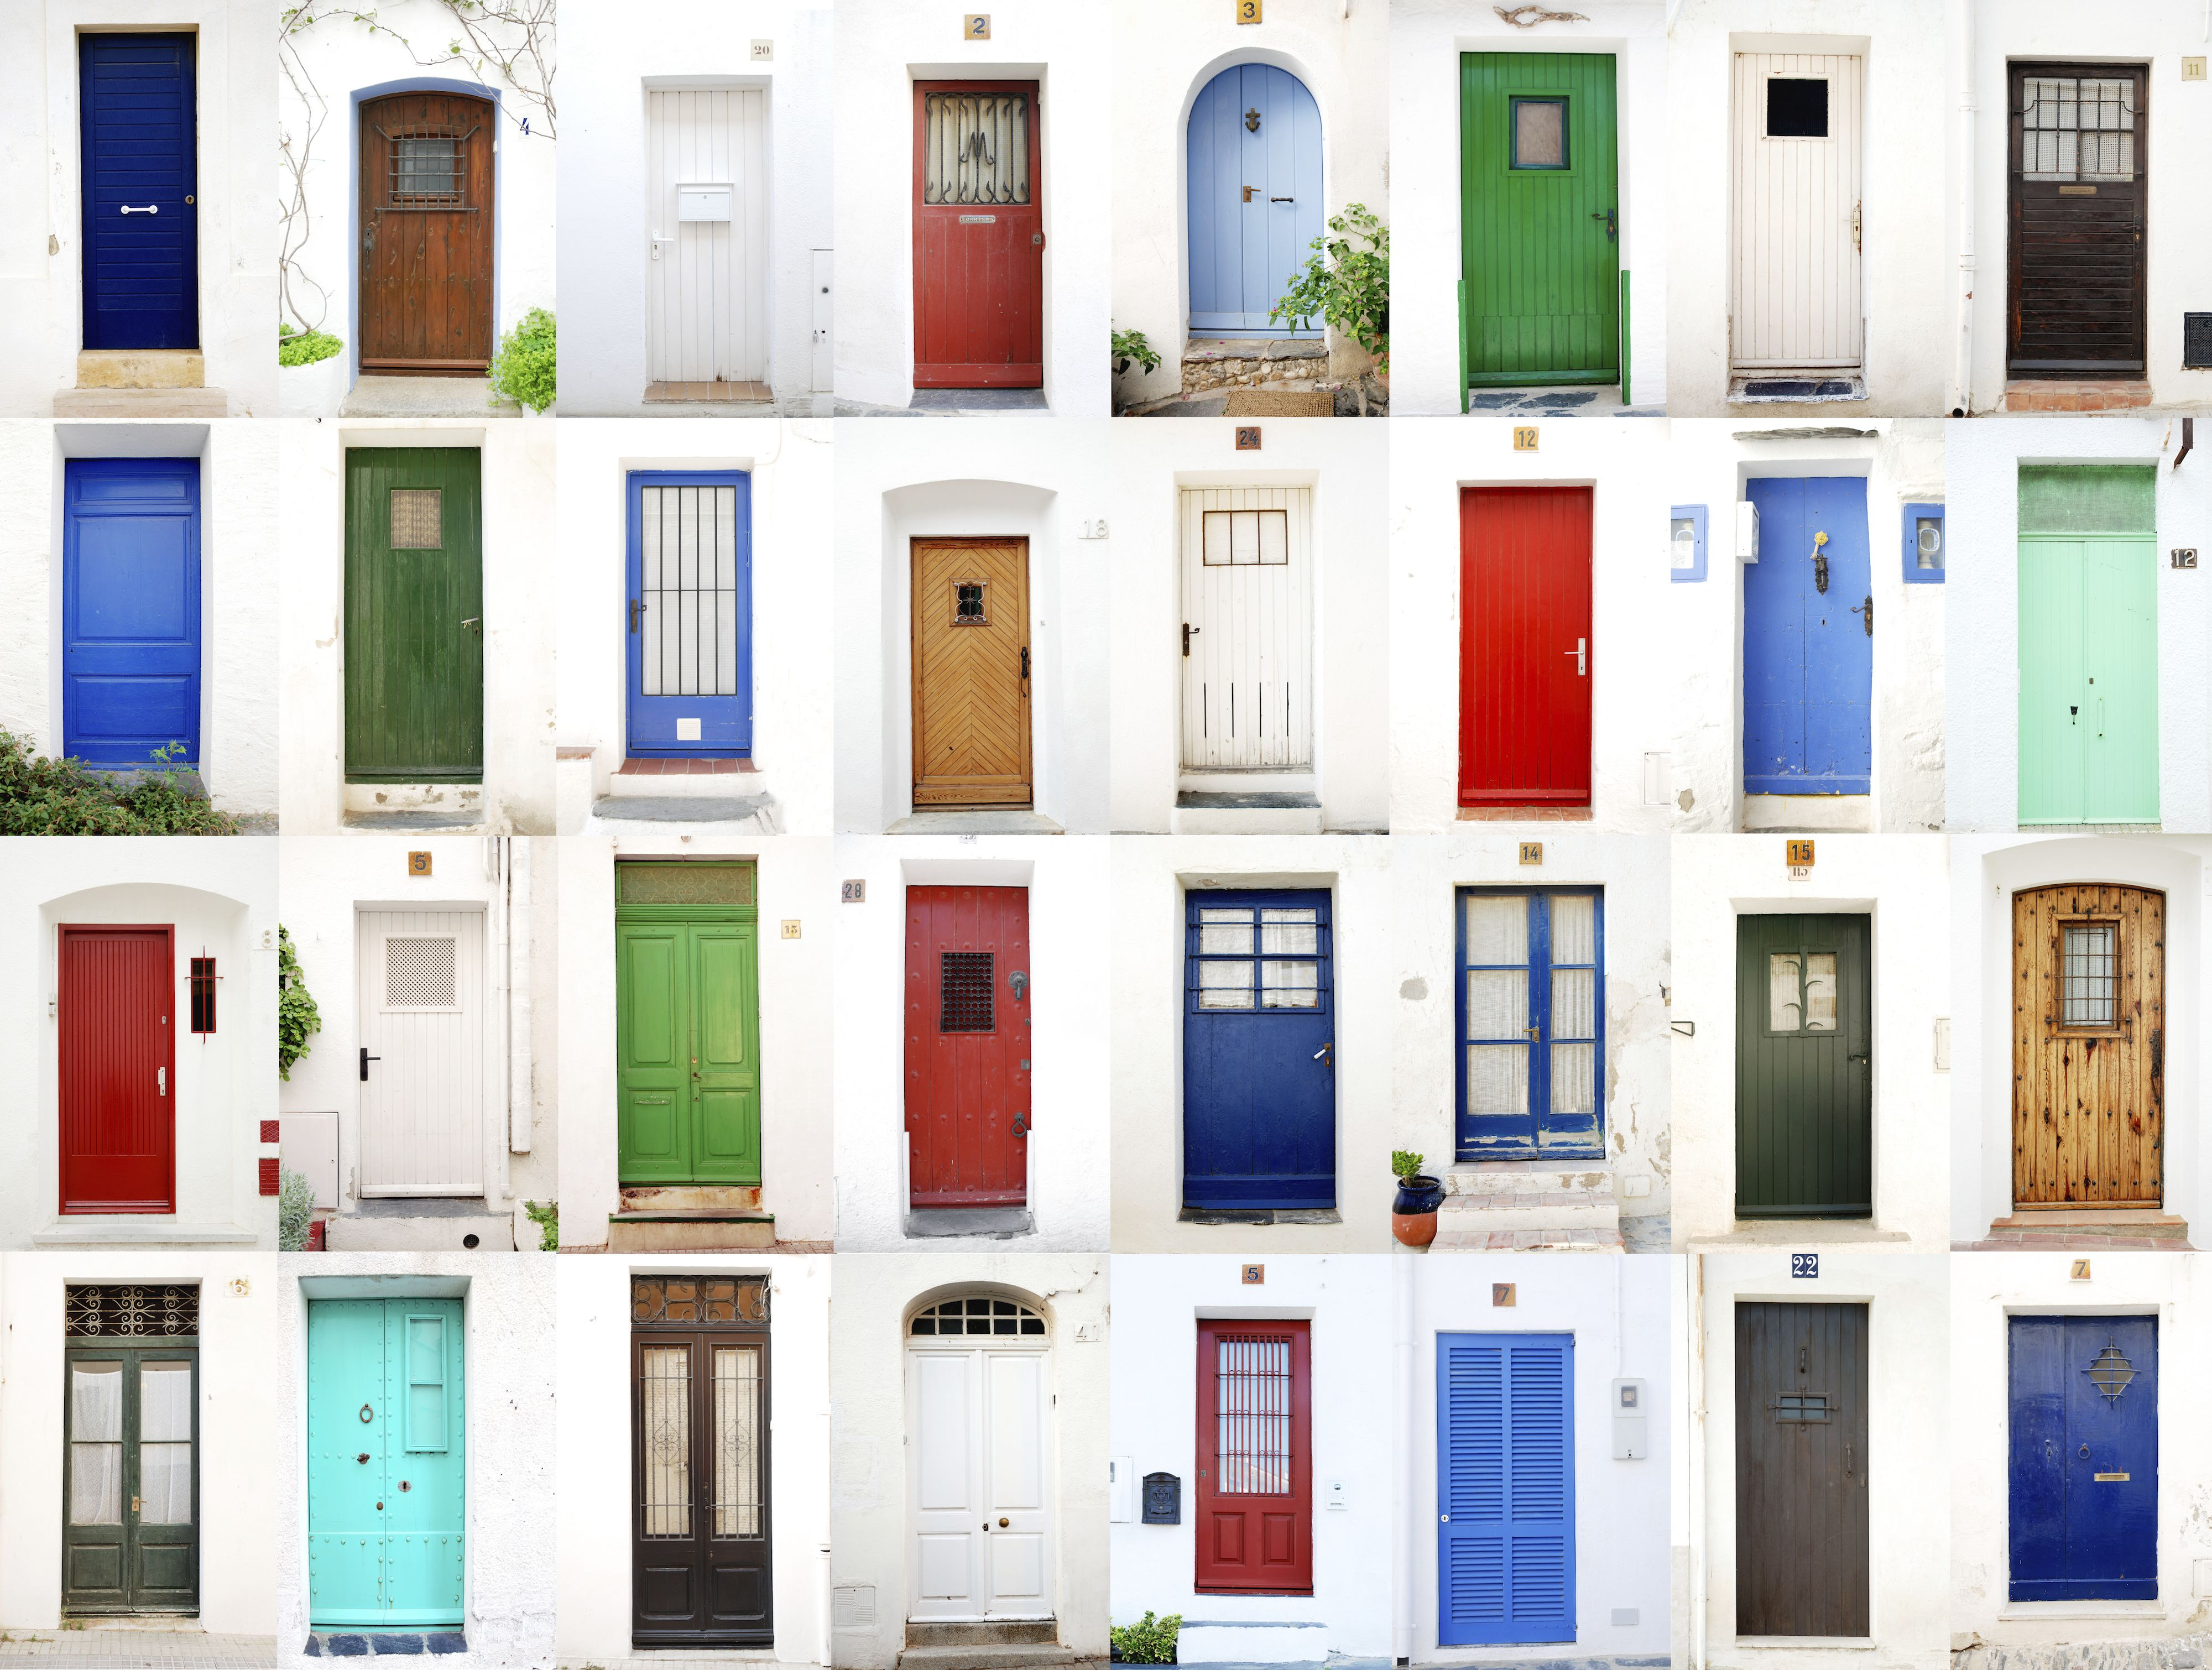
\includegraphics[width = \textwidth, height = .85\textheight, keepaspectratio]{figures/Doors.jpg}

\end{frame}

\note{
    Software communicate through ports. Imagine this as your computer having many doors to the internet and a program listening, waiting behind each of them.

    Your web browser is using a door, your e-mail client is using another, software updates come and go through yet another. Even Tiktok gets a door of its own.

    You often won't even realize the software you install opens up a new port (door) to your computer.

    A piece of malware, or a malicious actor can exploit the bugs in the software behind open ports to gain access to your device. So a combination of open ports and buggy software often creates trouble.

    As with any defensive scenario, the more openings you need to watch, the poorer your security. Therefore it is important to keep track of these doors.
}

\begin{frame}
    \frametitle{Firewalls}
    
    \centering

    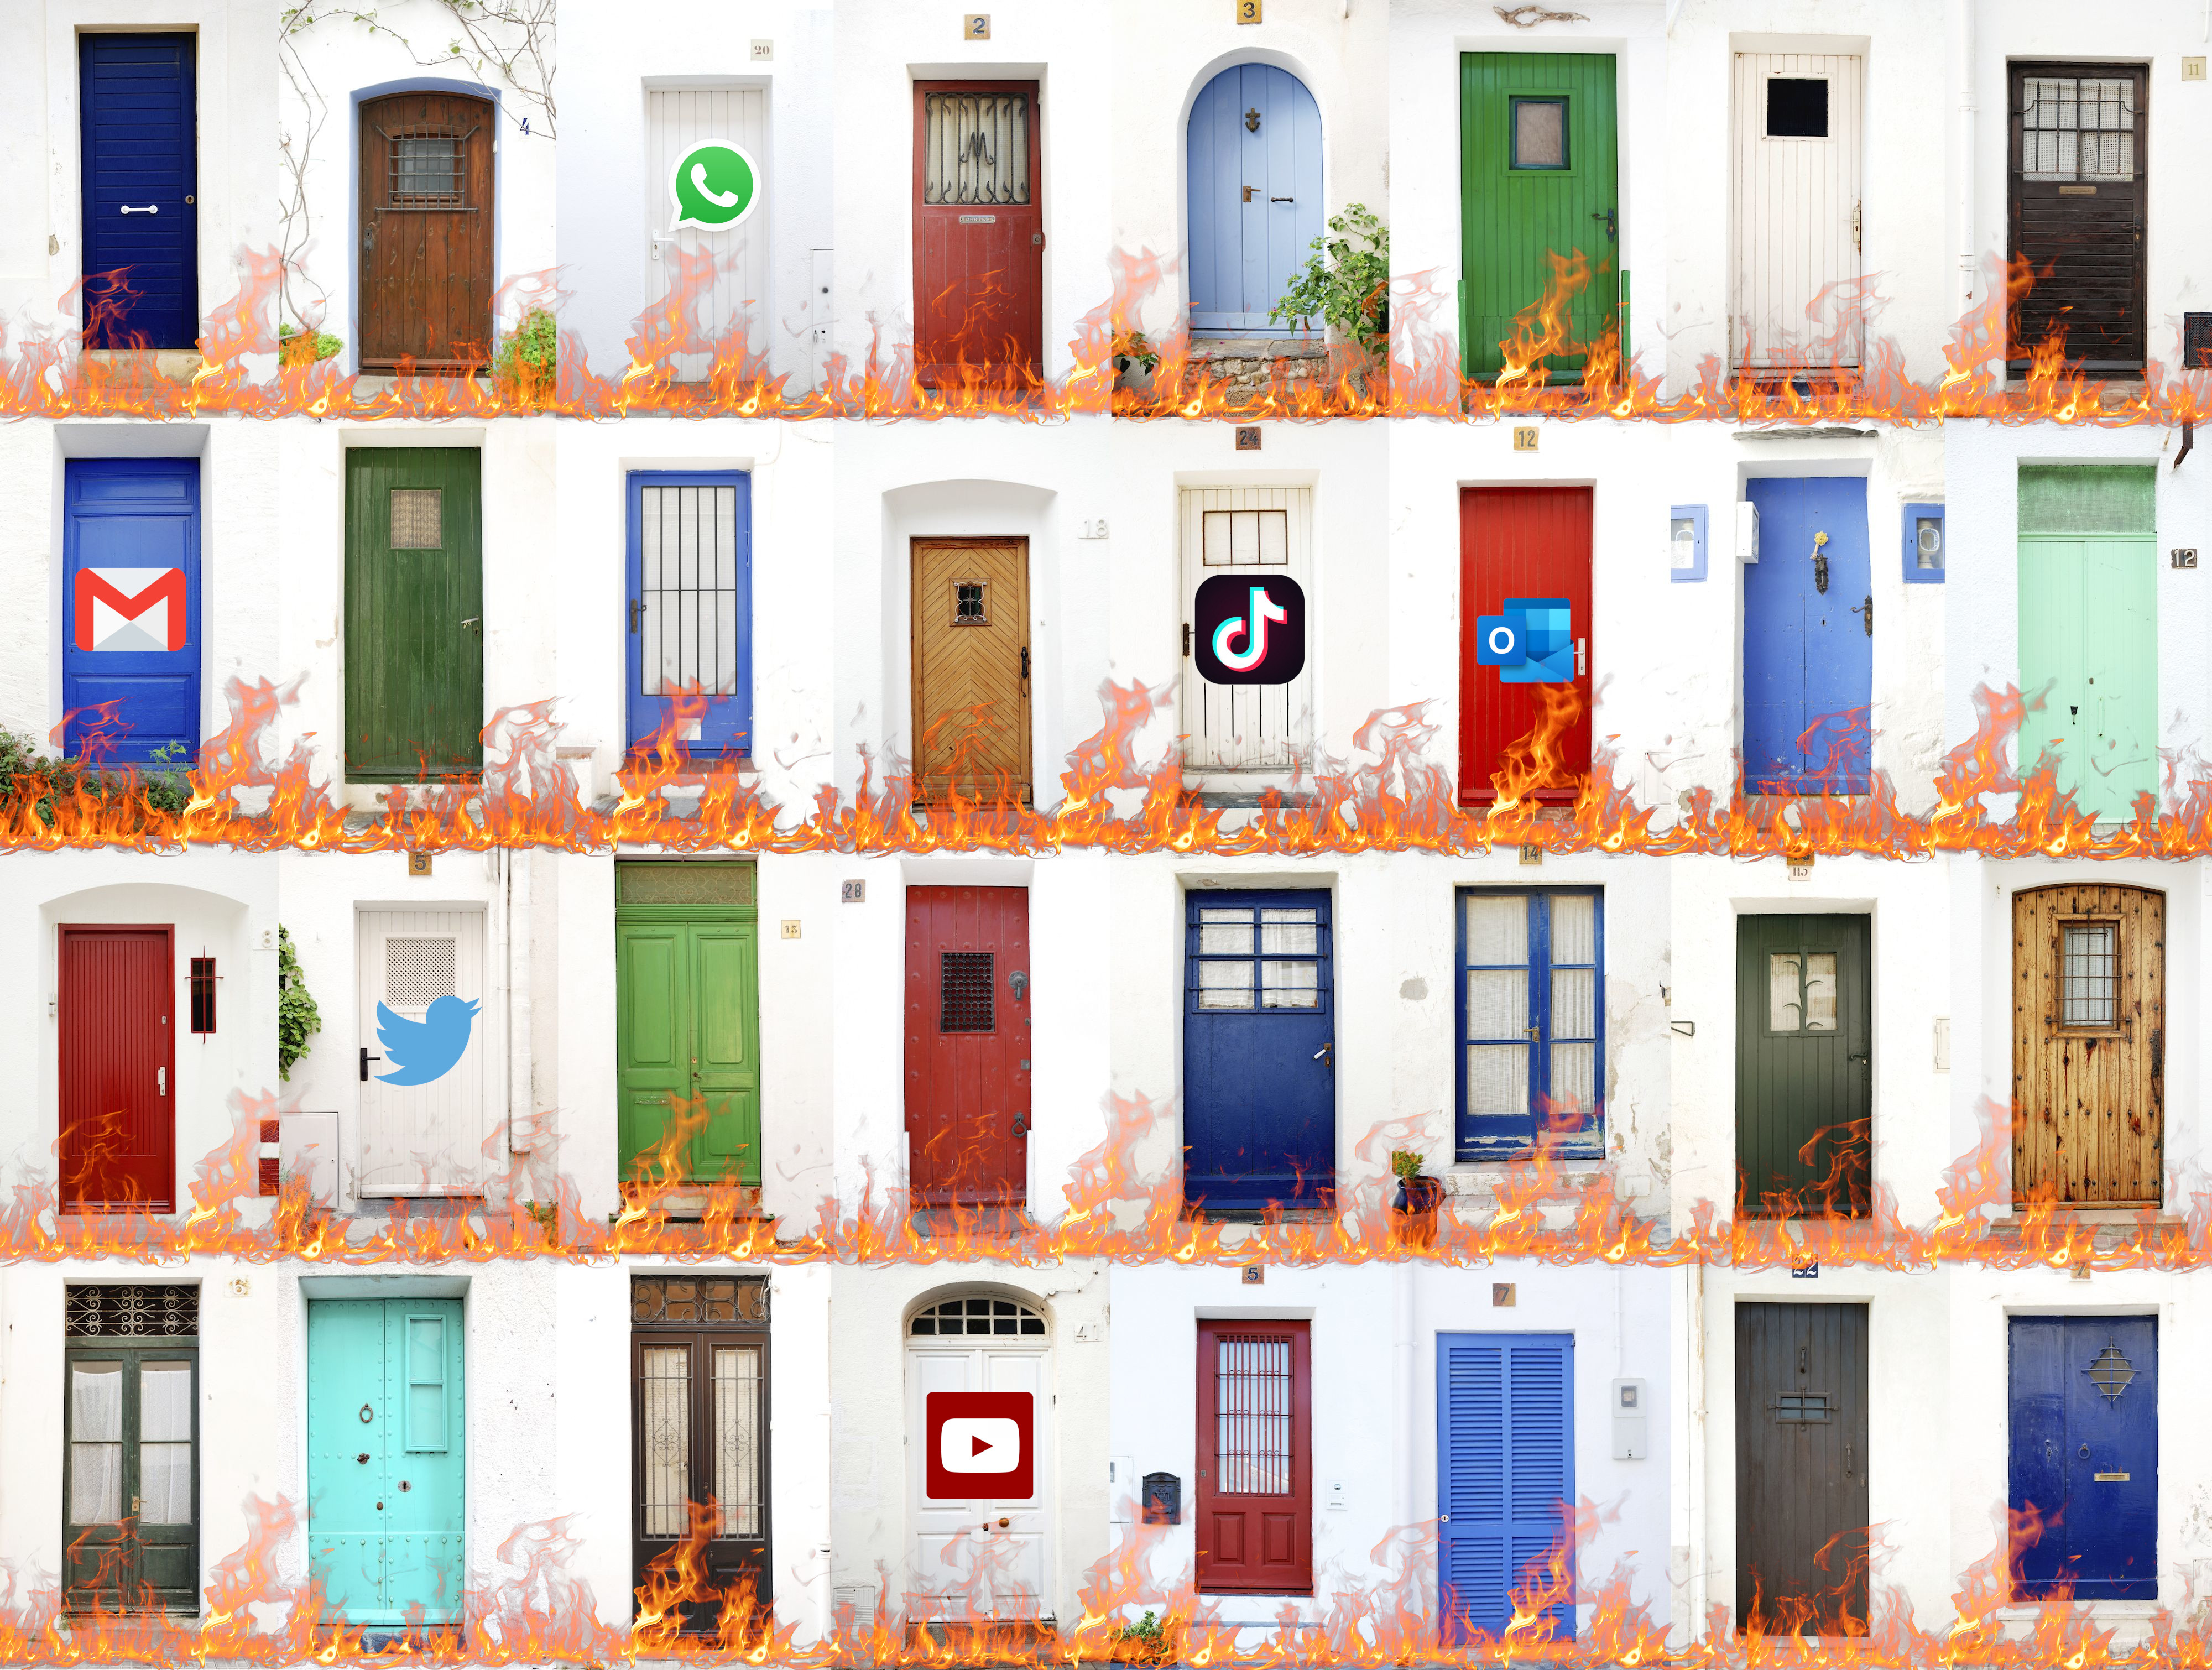
\includegraphics[width = \textwidth, height = .85\textheight, keepaspectratio]{figures/Firewall.jpg}

\end{frame}

\note{Despite the cool name, what a firewall does is more akin to a border control agent.

A firewall is a set of rules that define the admissable traffic for a device.

What port, what protocol, which direction, from where?

Denying traffic on ports you don't use or recognize can save you trouble down the road. The problem is, you may accidentally block legitimate traffic if you are not careful...
}

\begin{frame}
    \frametitle{In Short}
    
    \begin{itemize}
        \item Use Strong Passwords
        \item Don't Engage if You Didn't Initiate
        \item Update Your Software
        \item Remove Unnecessary Software from Your Life
        \item Use Anti-Virus
        \item Setup a Firewall
    \end{itemize}

\end{frame}


\end{document}
